\documentclass[fleqn,twoside,openright]{iofm_studentthesis}% remove option "german" for english version
% load definitions, i.e. some useful shortcuts and notational stuff for tensors etc.
%=========================================================================
% DEFINITIONS
%=========================================================================

% Anmerkung: \newcommand testet im Gegensatz zu \def darauf, ob ein
% Befehl bereits vorhanden ist und gibt ggf. eine Fehlermeldung aus
% so zum Beispiel
%\def\mc  #1{\mbox{$\mathcal   #1$}}
% im Vergleich zu
%\newcommand{\mc}[1]{\ensuremath{\mathcal{#1}}}

%=========================================================================

% units
\newcommand{\unit}[1]{\operatorname{#1}}


% % % % % % % % % % % % % % % % % % % % % % % % % % % % % % % % % % % % % % % % % % % % %
% % % % % % % % % % % % % % % % % % % % % % % % % % % % % % % % % % % % % % % % % % % % % 

%%
% Mathematical Operators
%%

% non-standard tensor operators
\newcommand{\Otimes}{\,\overline{\otimes}\,}
\newcommand{\Utimes}{\,\underline{\otimes}\,}
\newcommand{\norm}[1]{\|#1\|}
\newcommand{\dev}{\operatorname{dev}}
\newcommand{\trace}{\operatorname{tr}}
\def\tran{\mathrm{t}} % transposed

% derivatives
\newcommand{\Div}[1][\te X]{\nabla_{\!#1}\cdot}
\renewcommand{\div}[1][\te x]{\nabla_{\!#1}\cdot}
\newcommand{\Grad}[1][\te X]{\nabla_{\!#1}}
\newcommand{\grad}[1][\te x]{\nabla_{\!#1}}
\newcommand{\dd}[2][]{\frac{\mathrm{d}#1}{\mathrm{d}#2}}
\newcommand{\DD}[2][]{\frac{\mathrm{D}#1}{\mathrm{D}#2}}
\newcommand{\pp}[2][]{\frac{\partial#1}{\partial#2}}

% assembly-operator
\def\Ass{\mathop{\mathchoice{\AssX\huge}{\AssX\Large}{}{}}}
% helper for \Ass
\def\AssX#1{{\setbox0=\hbox{#1\sf\textbf{A}}\lower.2\ht0\copy0}}

%%%%%%%%%%%%%%%%%%%%%%%%%%%%%%%%%%%%%%%%%%%%%%%%%%%%%%%%%%%

\newcommand{\B}{\boldsymbol}
\newcommand{\sfA}{ {\textsf{A}} }
\newcommand{\BE}{{\textbf{\textsf{E}}}}
\newcommand{\BS}{{\textbf{\textsf{S}}}}
\newcommand{\E}{{{\textsf{E}}}}
\newcommand{\I}{{\textsf{I}}}
\newcommand{\Y}{{{\textsf{Y}}}}
\newcommand{\sfC}{{{\textsf{C}}}}
\newcommand{\sfS}{{{\textsf{S}}}}
\newcommand{\sfT}{{{\textsf{T}}}}
\newcommand{\BA}{{\textbf{\textsf{A}}}}
\newcommand{\BC}{{\textbf{\textsf{C}}}}
\newcommand{\BD}{{\textbf{\textsf{D}}}}
\newcommand{\BI}{{\textbf{\textsf{I}}}}
\newcommand{\BT}{{\textbf{\textsf{T}}}}
\newcommand{\be}{\begin{equation}}
\newcommand{\ee}{\end{equation}}
\newcommand{\bea}{\begin{eqnarray}}
\newcommand{\eea}{\end{eqnarray}}
\newcommand{\vareps}[0]{\varepsilon}
\newcommand{\mr}[1]{\mathrm{#1}}
\newcommand{\Mt}{{\mr{M}_\mr{t}}}
\newcommand{\Mc}{{\mr{M}_\mr{c}}}
\newcommand{\M}{{\mr{M}}}
\newcommand{\A}{{\mr{A}}}
\newcommand{\epspl}{\vareps_\mr{pl}}
\newcommand{\epstr}{\vareps_\mr{tr}}
\newcommand{\epstrdev}{\vareps_\mr{tr,dev}}
\newcommand{\epstrvol}{\vareps_\mr{tr,vol}}
\newcommand{\epsvol}{{\vareps_\mr{vol}}}
\newcommand{\epsdev}{{\vareps_\mr{dev}}}

\newcommand{\Eal}{{\textsf E}^\alpha}
\newcommand{\Evol}{{\textsf E}_\mr{vol}}
\newcommand{\Edev}{{\textsf E}_\mr{dev}}
\newcommand{\hatEvol}{\widehat{{\textsf E}}_\mr{vol}}
\newcommand{\hatEdev}{\widehat{{\textsf E}}_\mr{dev}}
\newcommand{\sigmac}{\B\sigma_\mr{mac}}
\newcommand{\half}{\frac{1}{2}}

\newcommand{  \Isym  }{  \BI^\mr{sym}  }
\newcommand{  \Idev  }{  \BI^\mr{dev}  }
\newcommand{  \Ivol  }{  \BI^\mr{vol}  }

%%%%%%%%%%%%%%%%%%%%%%%%%%%%%%%%%%%%%%%%%%%%%%%%%%%%%%%%%%%

%%
% Variable Typesets
%%

% define tensor notation
% mathchoice detects in which "surrounding" content will be placed. \mathchoice{displaystyle}{textstyle}{subscript}{subsubscript}. textstyle is inline, e.g. "normal vector $\te n$ some more text".
\makeatletter
\newcommand{\te}[1]{\mathchoice{\mbox{\boldmath$#1$}}{\mbox{\boldmath$#1$}}{\mbox{\let\f@size\sf@size\selectfont\boldmath$#1$}}{\mbox{\let\f@size\ssf@size\selectfont\boldmath$#1$}}}   % 1st order tensor
\newcommand{\tz}[1]{\mathchoice{\mbox{\boldmath$#1$}}{\mbox{\boldmath$#1$}}{\mbox{\let\f@size\sf@size\selectfont\boldmath$#1$}}{\mbox{\let\f@size\ssf@size\selectfont\boldmath$#1$}}}   % 2nd order tensor
\newcommand{\td}[1]{\mathchoice%
{% display style
    \dimen0=\f@size pt%
    \addtolength{\dimen0}{-\ssf@size pt}%
    \mbox{\raisebox{\the\dimen0}{$\scriptscriptstyle 3$}$\mathbb #1$}
}{% text style
    \dimen0=\f@size pt%
    \addtolength{\dimen0}{-\ssf@size pt}%
    \mbox{\raisebox{\the\dimen0}{$\scriptscriptstyle 3$}$\mathbb #1$}
}{% scriptstyle
    \let\f@size\sf@size\selectfont%
    \dimen0=\f@size pt%
    \addtolength{\dimen0}{-\ssf@size pt}%
    \mbox{\raisebox{\the\dimen0}{$\scriptscriptstyle 3$}$\mathbb #1$}
}{% scriptscriptstyle
    \let\f@size\ssf@size\selectfont%
    \mbox{\raisebox{1pt}{$\scriptscriptstyle 3$}$\mathbb #1$}
}}  % 3th order tensor
\newcommand{\tv}[1]{\mathchoice{\mbox{\boldmath$\mathsf #1$}}{\mbox{\boldmath$\mathsf #1$}}{\mbox{\let\f@size\sf@size\selectfont\boldmath$\mathsf #1$}}{\mbox{\let\f@size\ssf@size\selectfont\boldmath$\mathsf #1$}}}  % 4th order tensor

% define vectors and matrices
\newcommand{\vc}[1]{\mathchoice{\mbox{\underline{\boldmath$\mathrm{#1}$}}}{\mbox{\underline{\boldmath$\mathrm{#1}$}}}{\mbox{\let\f@size\sf@size\selectfont\underline{\boldmath$\mathrm{#1}$}}}{\mbox{\let\f@size\ssf@size\selectfont\underline{\boldmath$\mathrm{#1}$}}}}
\newcommand{\mx}[1]{\mathchoice{\mbox{\underline{\boldmath$\mathrm{#1}$}}}{\mbox{\underline{\boldmath$\mathrm{#1}$}}}{\mbox{\let\f@size\sf@size\selectfont\underline{\boldmath$\mathrm{#1}$}}}{\mbox{\let\f@size\ssf@size\selectfont\underline{\boldmath$\mathrm{#1}$}}}}
\makeatother

%%%%%%%%%%%%%%%%%%%%%%%%%%%%%%%%%%%%%%%%%%%%%%%%%%%%%%%%%%%

% psfrag-abkuerzungen
\newcommand{  \psr   }[1]{  \psfrag{#1}[r][r]{   ${\scriptstyle #1 \!\!}$ }  }
\newcommand{  \pst   }[1]{  \psfrag{#1}[t][t]{   ${\scriptstyle #1 }$ }  }
\newcommand{  \psrt  }[1]{  \psfrag{#1}[rt][rt]{ ${\scriptstyle #1 \!\!\!}$ }  }%

\RequirePackage{verbatim}
\let\trace\relax % trace already defined but newly defined in physics package, workaround
\RequirePackage{physics}

\author{Philipp Scherm} % set Author-Name (your name!)
\title{Multi Phase Modelling an Finite Element Implementation of Steel Heat Treatment} % your title
% choose type of your thesis
% Project Thesis (Bachelor) / Projektarbeit (Bachelor)
% Bachelor Thesis / Bachelorarbeit
% Project Thesis (Master) / Projektarbeit (Master)
% Master Thesis / Masterarbeit
\thesistype{Master Thesis}
% add all your supervisors with their full name
\addsupervisor{Prof.~Dr.-Ing.~habil.~Andreas~Menzel}
\addsupervisor{Markus Schewe,~M.~Sc.}

\begin{document}
%
\maketitle % Erstellt die Titelseite, welche oben durch Angabe von \author und \title noch angepasst werden kann
%
\addblankpage% add blank page (backside of title-page, only inserted for two-sided layout)
%
\thispagestyle{empty}
\begin{figure}
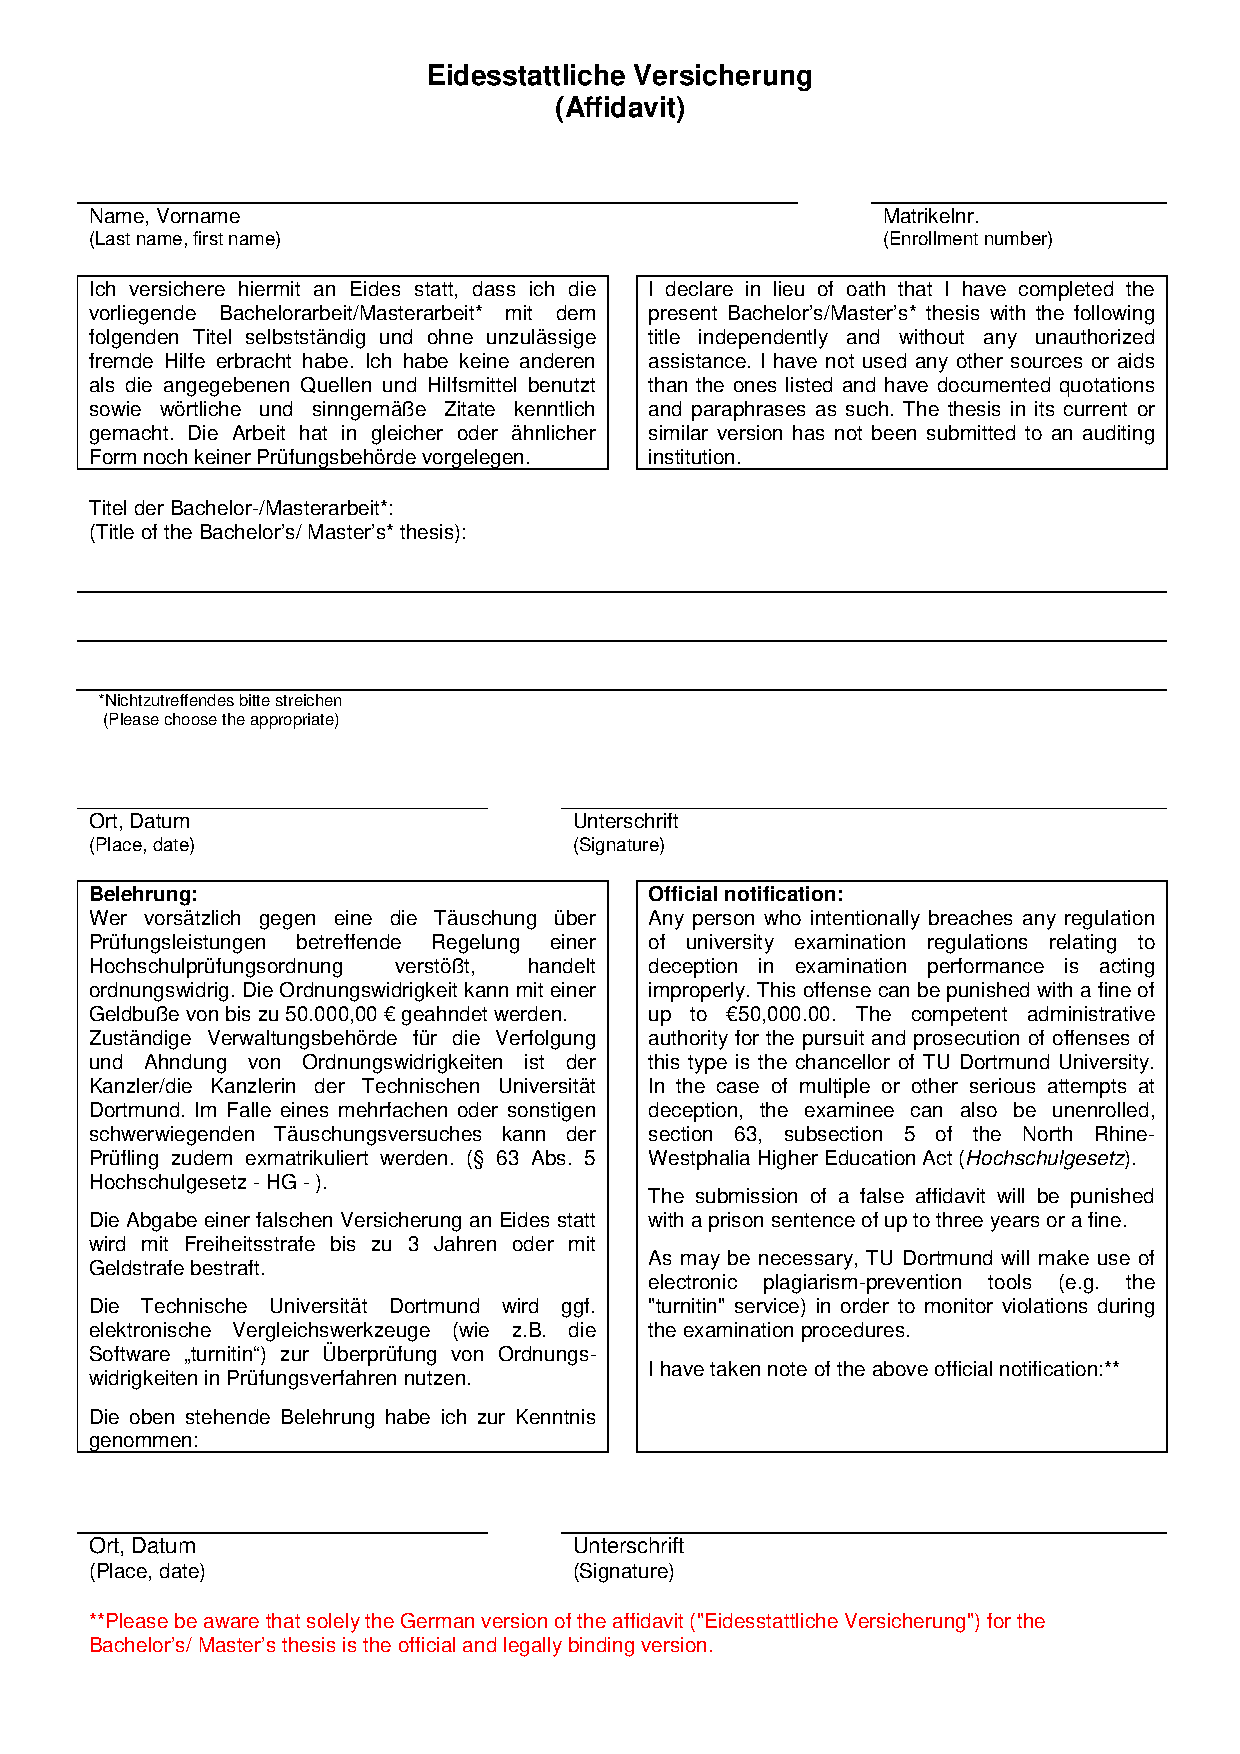
\includegraphics[width=1.0\textwidth,trim=1.3cm 0cm 1.2cm 0cm,clip]{Eidesstattliche_Versicherung} % Erstellt die zu unterschreibende Seite mit der Eidesstattlichen Versicherung
\end{figure}
%
\addblankpage% add blank page (backside of Eidesstattliche_Versicherung, only inserted for two-sided layout)
%
\setcounter{page}{1} % Startet Seitennummerierung bei 1
\tableofcontents % Erstellt Inhaltsverzeichnis
%
% Im Folgenden k�nnen die einzelnen Kapitel der Arbeit mittels \include eingef�gt werden

\chapter{Introduction}
\thispagestyle{fancy}
\label{chap:intro}


Heat treatment of metals as a way of altering it's properties and microstructure is a process known for millennia.  
For many millennia heat treatment of metals has been an important part of industrial development. The ancient egypts used annealing to 


The heat treatment process of steel usually involves vigorously heating the metal and throwing it into cold water. A later less vigorous reheating is optional. \textit{Maybe spare this for the presentation}



Define feat treatment 

talk about history islamic, egypt, india, china, 9000 years bc 

\chapter{Model/Theoretical Framework/Method}
\thispagestyle{fancy}
\label{chap:model}
Heat treatment problems require the solution of three problems. Heat transfer, mechanical material response and phase transformation are coupled by their physical interactions. 

\section{Metallurgy}
Heat treatment of steel aims to alter the microstructure in 

Influence on the decomposition of austenite by the cooling rate and path

The German standard \cite{din_en_10020_din_2000} defines steel in the most common form to be iron with a carbon content below 2\%. Depending on the microstructure different phases are distinguished. They are characterized by their chemical composition, crystal lattice and shape. These characteristics influence the macroscopical properties exhibited by steel like strength, toughness, hardness and ductility. In a heat treatment process the microstructure  and the properties can be altered. 
Here three different phases are of interest, austenite, pearlite, bainite and martensite. 
When steel is heated and held at a suffcient temperature and sufficient time it consists of stable and solid austenite. Austenite has a face-centered cubic lattice ($\gamma$-iron) with the an iron atom on every corner and at the center of each face. The carbon is dissolved in the interstitial spaces between the iron atoms. Austenite is the starting point of the modelled quenching process. \\ \\
Martensite was discovered by Floris Osmond and named after Adolf Martens in \cite{osmond_microscopic_1904}. It forms when austenite is quenched with a high cooling rate so that the diffusion of carbon out of the lattice is suppressed. 
Martensite exhibits a body-centered tetragonal structure and is supersaturated with carbon. The stretch from a cubic austenite structure to tetragonal martensite causes shear strains of a magnitude of 0.26, see \cite{bhadeshia_worked_2001}, and dislocations that lead to high hardness of martensite. From martensitic steel a Brinell hardness of 700 can be achieved while the maximum of a pearlitic structure is approximately 400 Brinell, c.f. \cite{eugene_a_avallone_iron_2007}. \\

In \cite{cohen_martensite_1992} the martensite transformation is described as being of displacive nature, accompanied by a change in the crystal lattice. In steel it is athermal. There is no thermal activation, e. g. incubation time and no time dependence. 

The transformations starts at the martensite start temperature $M_S$ and is driven by cooling until the martensite finish temperature $M_F$ is reached. The transformation is only driven by cooling and not by the time spent below $M_S$.  If there is no further cooling the transformation stops. It is possible for a material cooled to room temperature to retain austenite if the $M_F$ temperature is below room temperature. \\
In iron-alloys without carbon martensite transformation occurs isothermally. 

When not quenched quickly enough to suppress it, diffusion of carbon occurs below the temperature $A_3$. With decreasing temperature, the carbon-solubility of austenite drops and carbon diffuses out of the lattice. The carbon-depleted structure turns into ferrite which is almost pure iron with a body-centered cubic lattice ($\alpha$). The locally carbon-enriched neighbouring structure turns into perlite. Perlite is a mixture of 87.5 wt\% ferrite and 12.5 wt\% carbide in lamellar structure that forms below the temperature $A_1$. By the diffusion of carbon the struxture is alternatingly locally carbon-enriched and depleted. In the depleted parts ferrite forms while the enriched structure turns into cementite. Cementite is a chemical compound of iron and steel $FE_3C$. 
The lamellae structure is similar to that of mother-of-pearl which gives the steel phase it's name. 

While there are views that bainite is formed in a reconstructive way \cite{bhadeshia_bainite_1990}, in this thesis the bainite formations is regarded as displacive \cite{bhadeshia_bainite_2019}
Below a temperature of about 580°C reconstructive transformation is virtually non-existent because iron and alloying atoms are virtually immobile while carbon still solutes. \cite{christian_simple_1990} 
-\> bainte start temperature

Bainite is formed below the bainite start temperature $B_S$ when the matrix atoms of the lattice are virtually immobile while the carbon atoms are still in solution. 
Upper bainite above $M_S$ lower bainite below it. 

Differentiation of the transformations in reproductive-displacive and athermal-isothermal \cite{bhadeshia_bainite_1990} 


\section{Phase Transformations}

Within this work two different kind of phase transformations are treated. Martensite transformation is athermal without thermal activation while the transformation into bainite is diffusion controlled. The bainite transformation is time dependent while martensite transformation is only driven by cooling, c.f. \cite{totten_steel_2007}. \\
%%%%%%%%%%%%%%%%%%%%%%%%%%%%%%%%%%%%%%%%%%5

For the microstructural problem two different widely accepted (sources!!!) phenomenological models are used.\\
The martensite transformation relies on the Koistinen-Marburger model established by \cite{koistinen_general_1959}. It describes the transformtion using the following equation \\\\

-----------------------------------------------------
As dargelegt in the previous chapter athermal and diffusion-controlled phase transformations are treated in this thesis. In athermal transformations there is no thermal activation, e. g. incubation time and no time dependence. The transformation is purely driven by cooling. If there is no further cooling the transformation stops. The transformation from austenite to martensite is regarded as being athermal. It's modelling relies on the Koistinen-Marburger model established in \cite{koistinen_general_1959}. It describes the evolution of the volume fraction of martensite $\beta_M$ that is also depicted in fig. \ref{fig:MartDevelop} using the following equation 
\begin{equation}
	\beta_M =  1 - e^{-k\,(M_S - T)} \quad. \label{eq:KM}
\end{equation}
The parameter $k$ is material specific and describes the speed of the transformation. The martensite starting temperature $M_S$ depends on the material and the other factors as the local carbon content that can be influenced by other phase transformations \ref... It determines the temperature at which the transformation starts. The transformation is regarded as complete when the martensitic volume fraction reaches $99\%$. The martensite finish temperature $M_F$ can be calculated by rearranging \ref{eq:KM} and inserting $\beta_M = 99\%$.\\
\begin{figure}[h]%[h]
\centering
\psfragfig[ trim = 0 0 0 0, clip = true]{figs/MartDevelopment} 
\caption{Development of the martensite volume fraction under cooling.}
\label{fig:MartDevelop}
\end{figure}
The rate of the martensite transformation can be described by 
\begin{equation}
	\dot{\beta}_M = -e^{-k\left[M_S-T\right]} \,k \, \dot{T} = \left[ 1-e^{-k\left[M_S-T\right]} - 1 \right] k \, \dot{T} = - \left[ 1-\beta_M \right] k \, \dot{T} \quad. 
\end{equation}
While this equation is valid when only considering the transformation from austenite to martensite it can be generalized for the usage with more phase transformations by interpreting the term $1-\beta_M$ as the remaining austenite $\beta_A$ available for transformation. This yields the following rate for the evolution of the martensitic phase
\begin{equation}
	\dot{\beta}_M = - \beta_A \, k \, \dot{T} \quad. \label{eq:rateKM}
\end{equation}

The other transformation considered in this thesis is regarded as diffusion-controlled with thermal activation. There is a time-dependence in these transformations and they do continue isothermally when the cooling is stopped \ref... The transformation from austenite to bainite falls into this category. Schlecht.  \\
Diffusional processes and transformations are often modelled using the...
The equation used to describe this transformation is the JMAK law developed by Johnson, Mehl, Avrami and Kolmogorov (Avrami, 1940; Cahn, 1956) which is only valid for isothermal transformations. 
The JMAK law 
\begin{equation}
	\beta_B = \hat{\beta}_B\,[1-e^{-b_B\,(t^{N_B})}] \label{eq:JMAK}
\end{equation}
can be used for various diffusional transformations and other time dependent processes. \cite...
Here it is used to model the development of the volume fraction of bainite $\beta_B$ where $\hat{\beta}_B$ is the maximal amount of bainite reached in the transformation. Irgendwas mit  $\hat{\beta}_B = \beta_A + \beta_B$

with the maximal volume fraction of bainite $\hat{\beta}_B = \beta_A+\beta_B$  that can be reached if all austenite  and the
yields sigmoidal shapes seen in fig. \ref{fig:ficTime} with a slow start and a slow finish of the transformation but a high rate in between.
The parameters 
\begin{align}
	N_B(T) = \frac{6.1273}{\ln(\frac{t_B^f}{t_B^s})}\,\quad \text{and} \quad b_B(T) = \frac{0.01005}{(t^s_B)^{N_B(T)}}
\end{align}
are derived using the starting and finishing time $t_B^s$ and $t_B^f$ for the diffusive transformation. Those are defined at volume fraction of $1\%$ and $99\%$ of the target phase. The parameters are temperature dependent and can be determined from experimental TTT diagrams (Diss Yu 1977 oder so). \\
The time derivation of the JMAK law eq. \ref{eq:JMAK} yields the rate equation for isothermal cooling
\begin{equation}
	\dot{\beta}_B = \hat{\beta}_B\,b_B\,N_B\,t^{(N_B-1)}\,[1-\beta_B] \quad. \label{eq:ABrate0}
\end{equation}


% Adaption of JMAK law for anisothermal
As the JMAK law---and TTT-diagrams from which the parameters are derived---is only valid for isothermal transformations 
it has to be adapted to depict a cooling process. \\ 



In \cite{scheil_anlaufzeit_1935} a theory of the additivity of fractional nucleation is proposed to predict the start of the transformation from austenite during cooling.  The so-called `additivity rule' states that transformation starts when the fractions of nucleation $\frac{\Delta t_i}{\tau(T_i)}$ accumulated during the cooling reaches unity
\begin{equation}
	\int^{T_{x}}_{T_{0}} \frac{\dd{t}}{\tau(T)} = 1 \quad. %\approx \sum_{i=0}^{t_x} \frac{\Delta t_i}{\tau(T_i)} \quad
\end{equation}
$T_{0}$ is an equilibrium temperature at which no nucleation happens, $T_{x}$ is the temperature at which the transformation starts when following an anisothermal temperature path and $\tau(T)$ is the incubation time after that transformation starts for an isothermal temperature path. This means for a discretized calculation that the transformation starts when the fractions of nucleation at every time increment $\frac{\Delta t_i}{\tau(T_i)}$ amassed during the cooling reaches unity as follows
\begin{equation}
	\sum_{}^{} \frac{\Delta t_i}{\tau(T_i)} = 1 \quad.
\end{equation}
This empirical relation is used in \cite manningloring, wever to relate the starting time of transformation from isothermal and anisothermal. 
Pumphrey predicts the hardness of specimens after continuous and step-wise cooling 

Different criteria and conditions have been proposed for the additivity of a transformation. 
Cahn and Avrami call it isokinetic when nucleation and growth rate are proportional at the same phase composition. The development of a phase at two different transformations is the same besides a time factor. In a logarithmic plot they look identical with the slower one shifted to the right side. 
directly quote Hollomon?? 

This equals to a condition 

\begin{equation}
	\dot{beta} = g(\beta)\,h(T)
\end{equation}
Cahn proposes a less strict condition 
\begin{equation}
	\dot{beta} = f(\beta,T)
\end{equation}
that is 



It is shown in \cite{lusk_rule_1997} and \cite{christian_formal_2002} that this holds true for transformations that are isokinetic, c.f. \cite{cahn_transformation_1956}, and whose rate can be expressed in the following form 
\begin{equation}
	\dot \beta = h(\beta)\, g(T)
\end{equation}
like eq. \ref{eq:ABrate0}.

Based on the additivity rule \cite{tzitzelkov_mathematische_1974} developed an algorithm to predict the phase development for continuous cooling. 
For this the cooling curve 
A continuous temperature curve can be discretized into isothermal increments as in fig. \ref{fig:discCoolCurve}. 

\begin{figure}[h]%[h]
\centering
\psfragfig[ trim = 0 0 0 0, clip = true]{figs/discretizedCoolingCurve} 
\caption{Continuous and incrementally isothermal discretized cooling curve.}
\label{fig:discCoolCurve}
\end{figure}



The cooling curve is discretized into small isothermal steps at declining temperatures. Every step $i$ is defined by it's temperature $T_i$ and it's duration $\Delta t_i$. \\
In the following the procedure is explained using two isothermal steps of $\Delta t = 1.5s$ at the temperatures  $T1 = 600^\circ C$ and $T2 = 550^\circ C$. \\ 
The first step starts at P0 with a volume fraction of bainite 
$\beta_B = 0$ and ends at P1 after $\Delta t$ at $\beta_B^1 = 0.17$ following the transformation curve for T1.  
For the next step at T2, a fictitious point P1$^\ast$ is introduced. It is the intersection of $\beta_B = \beta_B^1$ with the transformation curve for T2. The time will be called ficitious time $t^\ast$. It is the time transformation at T2 would take to yield $\beta_B^1$.\\
Then transformation is again  following the curve for $T2$ for a $\Delta t$ of 1.5s finishing at a volume fraction $\beta_B$ of 0.78. \\


% Grafik aus phasenumwandlung_beispiele_MS.ipynb weit unten
\begin{figure}[h]
\centering
\psfragfig[ trim = 0 0 0 0, clip = true]{figs/fictitiousTimeSteps} %width = 0.7\textwidth,
\caption{Two isothermal cooling steps.}
\label{fig:ficTime}
\end{figure}

\begin{figure}[h]
\centering
\psfragfig[width = 0.3\textwidth, trim = 0 0 0 0, clip = true]{figs/isothermalStepsTt} 
\caption{Discretized example cooling curve.}
\label{fig:discTt}
\end{figure}

\begin{figure}[h]
\centering
\psfragfig[ trim = 0 0 0 0, clip = true]{figs/isothermalSteps} %width = 0.9\textwidth,
\caption{}
\label{fig:}
\end{figure}



% include more graphics 

To incorporate the fictitious time into the rate equation the steps laid out in (Reti 2001) are done. Using the JMAK law \ref{eq:JMAK}, the fictitious time for a given volume fraction $\beta_B$ and a temperature $T$ the fictitious time $t^\ast$ is derived as 
\begin{equation}
	t^\ast = \left( \frac{\ln A}{b(T_{i+1})}\right)^\frac{1}{N(T_{i+1})}, \quad A = \frac{\hat{\beta}}{\hat{\beta}-\beta_i}  \quad.
\end{equation}
This relation then is inserted into the rate equation \ref{eq:ABrate0} to replace the isothermal transformation time and eliminate the explicit time dependence 
\begin{equation}
	\dot{\beta} = N\,b^{\frac{1}{N}}\,(\hat{\beta}-\beta)\,\left(\ln A \right)^{1-\frac{1}{N}}\quad. \label{eq:ABrate}
\end{equation}
The generalization of the rate equation for more phases \textit{works similar} to the generalization of the martensitic rate. The maximal volume fraction of bainite $\hat{\beta}$ in (Oliviera 2010) is interpreted as 
\begin{equation}
	\hat{\beta} = \beta_A + \beta_B = 1 - \beta_M \quad. 
\end{equation}
This leads to a desired coupling of the rate equations of Bainite and Martensite. \\\\





\subsection{Involved Phases}
Floris Osmond named Martensite after Adolf Martens in \cite{osmond_microscopic_1904}

\subsection{phenomenological models}
Kostinen Marburg

JMAK 


Bringe ich die Metallurgie in dieses Kapitel und mische sie mit den Gleichungen oder trenne ich es in zwei Kapitel? 


\section{Thermal Problem}

The thermal problem is governed by the heat equation 


\section{mechanical}
The heat treatment problem is solved for small strains. The strain measurement is defined as 
\begin{equation}
	\varepsilon = \frac{1}{2}\left( \nabla_x u + [\nabla_x u]' \right)
\end{equation}
with $u$ being the displacement. The mechanical problem is governed by the balance of linear momentum 
\begin{equation}
	\nabla_x \sigma = 0 \quad. 
\end{equation}
The equations are now discretized and 
\chapter{Algorithmic implementation}
\thispagestyle{fancy}
\label{chap:algo}


After establishing the rate equations for the phase transformations \ref{eq:ABrate} and \ref{eq:rateKM} in the previous chapter \ref{chap:model} there are modifications and regularisations necessary before one is able to use them for computation. For both equations a term $\zeta$ is introduced that controls whether transformation is happening or not, cf. \cite{pacheco_analysis_2001} and \cite{de_oliveira_thermomechanical_2010}. \\
For the martensite transformation $\zeta_{A \rightarrow B}$ contains two heaviside functions $\Gamma$ and a regularized step function using a $\tanh$. The first heaviside function $\Gamma(-\Delta\,T)$ ensures irreversibility and that transformation only occurs during cooling. The second heaviside function $\Gamma(T-M_F)$ prevents transformation below the martensite finish temperature. The regularized step function $\tanh(A\*(M_S-T))/2 + 1/2$ starts the transformation after the temperature is blow the martensite starting temperature. The regularization deals with the discontinuity of the transformation rate at $T=M_S$. The influence of $A$ is depicted in fig. \ref{fig:tanHPara}.
\begin{figure}[h]
\centering
\psfragfig[ trim = 0 0 0 0, clip = true]{figs/tanHPara} %width = 0.9\textwidth,
\caption{Regularized step function using a tanh with different parameters.}
\label{fig:tanHPara}
\end{figure}
 The choice of $A=1$ makes the effect of the regularization disappear ($< 1e-6$) at $M_S \pm 2\%$. \\
This yields the extended rate equation for the evolution of the martensitic volume fraction
\begin{align}
	\dot{\beta}_M &= - \zeta_{A \rightarrow M} \, \beta_A \, k \, \dot{T}  \\
	\text{with } \zeta_{A \rightarrow M} &= \Gamma(-\Delta\,T)\,\Gamma(T-M_F)\, (\tanh(A\*(M_S-T))/2 + 1/2) \quad. 
\end{align}


For the bainite transformation a new local time scale for every material point is introduced. The transformation time $\tau$ starts once the temperature at the material point drops below the bainite starting temperature $T_B^s$. This time scale is used to account for vastly different incubation times at different temperatures. The incubation time is regarded as the time on the left of the bainite starting time $t_B^s$ when looking at the TTT Diagram in fig. \ref...


The time on the left of the bainite starting time $t_B^s$ when looking at the TTT Diagram in fig. \ref... is regarded as incubation time. The incubation time $\tau$ necessary to start the transformation is vastly different at different temperatures. To account for this in a similar way to the anisothermal evolution of bainite, Scheill's additivity \cite... is used to determine when $t_B^s$ is reached following a cooling curve. \\
The following condition is checked at every time step after an update of $\tau$ to determine the start of the transformation
\begin{gather}
	\tau = \tau + \frac{\Delta T}{t_B^s} \\
	t_B^s \geq \ \tau \quad.
\end{gather}




The initial value problem represented by the rate equations is solved by implicit time integration which leads to the evolution equation $\beta^{n+1} = \beta^n + \Delta \beta^{n+1}, \quad \text{with  } \Delta \beta^{n+1} = \Delta t \, \dot{\beta}^{n+1}$. \\
After bringing these equations into residual form 
\begin{align}
	\begin{split}
		\vc {R_{\beta}} &= \vc \beta^{n+1} - \vc \beta^n- \vc {\Delta \beta} \\
		&= \begin{bmatrix}
			R_{\beta_B}\\ 
			R_{\beta_M}
		\end{bmatrix} 		
		= \begin{bmatrix}
			\beta_B^{n+1} - \beta_B^{n} - \Delta \beta_B^{n+1} \\ 
			\beta_M^{n+1} - \beta_M^{n} - \Delta \beta_M^{n+1}
		\end{bmatrix}
	\end{split} \label{eq:betaRes}
	\\
	&\text{with  } \vc {\Delta \beta} = f(\vc \beta^{n+1})
\end{align}
the backward Newton method is used to solve the equation system \ref{eq:betaRes}. The update of the backward Newton 
\begin{equation}
	\vc \beta^{k+1} = \vc \beta^k - \frac{\vc {R_\beta}}{\vc {R_\beta \prime}}
	\label{eq:NewtonUpdate}
\end{equation}
with the iteration counter $k$ requires the derivation of the tangent 
\begin{gather}
	\vc {R_\beta \prime} = 
	\begin{bmatrix}
		\pdv{R_{\beta_B}}{\beta_B}&\pdv{R_{\beta_B}}{\beta_M}\\
		\pdv{R_{\beta_M}}{\beta_B}&\pdv{R_{\beta_M}}{\beta_M}\quad \text{with}\\ 
	\end{bmatrix}\\
	\pdv{R_{\beta_B}}{\beta_B} = 1 - \Delta t \,b^{\frac{1}{N}}\, N \left[B^{1-\frac{1}{N}} 
		- \left(1- \frac{1}{N}\right)\,B^{-\frac{1}{N}}\, \right] \\
	\pdv{R_{\beta_B}}{\beta_M} = 
		- \Delta t \,b^{\frac{1}{N}}\, N 
		\left[B^{1-\frac{1}{N}} 
		- \left(1- \frac{1}{N}\right)\,B^{-\frac{1}{N}}\,\left(1- \frac{\beta_A}{1-\beta_M}\right)
		\right]\\
	\pdv{R_{\beta_M}}{\beta_B} = -k\,\Delta T \, \zeta_{A \rightarrow M}\\
	\pdv{R_{\beta_M}}{\beta_M} = 1 - k\,\Delta T \,\zeta_{A \rightarrow M} \quad.
\end{gather}


\section{Implementation in Abaqus}
%% \documentclass{article}% remove option "german" for english version
% % load definitions, i.e. some useful shortcuts and notational stuff for tensors etc.
% %=========================================================================
% DEFINITIONS
%=========================================================================

% Anmerkung: \newcommand testet im Gegensatz zu \def darauf, ob ein
% Befehl bereits vorhanden ist und gibt ggf. eine Fehlermeldung aus
% so zum Beispiel
%\def\mc  #1{\mbox{$\mathcal   #1$}}
% im Vergleich zu
%\newcommand{\mc}[1]{\ensuremath{\mathcal{#1}}}

%=========================================================================

% units
\newcommand{\unit}[1]{\operatorname{#1}}


% % % % % % % % % % % % % % % % % % % % % % % % % % % % % % % % % % % % % % % % % % % % %
% % % % % % % % % % % % % % % % % % % % % % % % % % % % % % % % % % % % % % % % % % % % % 

%%
% Mathematical Operators
%%

% non-standard tensor operators
\newcommand{\Otimes}{\,\overline{\otimes}\,}
\newcommand{\Utimes}{\,\underline{\otimes}\,}
\newcommand{\norm}[1]{\|#1\|}
\newcommand{\dev}{\operatorname{dev}}
\newcommand{\trace}{\operatorname{tr}}
\def\tran{\mathrm{t}} % transposed

% derivatives
\newcommand{\Div}[1][\te X]{\nabla_{\!#1}\cdot}
\renewcommand{\div}[1][\te x]{\nabla_{\!#1}\cdot}
\newcommand{\Grad}[1][\te X]{\nabla_{\!#1}}
\newcommand{\grad}[1][\te x]{\nabla_{\!#1}}
\newcommand{\dd}[2][]{\frac{\mathrm{d}#1}{\mathrm{d}#2}}
\newcommand{\DD}[2][]{\frac{\mathrm{D}#1}{\mathrm{D}#2}}
\newcommand{\pp}[2][]{\frac{\partial#1}{\partial#2}}

% assembly-operator
\def\Ass{\mathop{\mathchoice{\AssX\huge}{\AssX\Large}{}{}}}
% helper for \Ass
\def\AssX#1{{\setbox0=\hbox{#1\sf\textbf{A}}\lower.2\ht0\copy0}}

%%%%%%%%%%%%%%%%%%%%%%%%%%%%%%%%%%%%%%%%%%%%%%%%%%%%%%%%%%%

\newcommand{\B}{\boldsymbol}
\newcommand{\sfA}{ {\textsf{A}} }
\newcommand{\BE}{{\textbf{\textsf{E}}}}
\newcommand{\BS}{{\textbf{\textsf{S}}}}
\newcommand{\E}{{{\textsf{E}}}}
\newcommand{\I}{{\textsf{I}}}
\newcommand{\Y}{{{\textsf{Y}}}}
\newcommand{\sfC}{{{\textsf{C}}}}
\newcommand{\sfS}{{{\textsf{S}}}}
\newcommand{\sfT}{{{\textsf{T}}}}
\newcommand{\BA}{{\textbf{\textsf{A}}}}
\newcommand{\BC}{{\textbf{\textsf{C}}}}
\newcommand{\BD}{{\textbf{\textsf{D}}}}
\newcommand{\BI}{{\textbf{\textsf{I}}}}
\newcommand{\BT}{{\textbf{\textsf{T}}}}
\newcommand{\be}{\begin{equation}}
\newcommand{\ee}{\end{equation}}
\newcommand{\bea}{\begin{eqnarray}}
\newcommand{\eea}{\end{eqnarray}}
\newcommand{\vareps}[0]{\varepsilon}
\newcommand{\mr}[1]{\mathrm{#1}}
\newcommand{\Mt}{{\mr{M}_\mr{t}}}
\newcommand{\Mc}{{\mr{M}_\mr{c}}}
\newcommand{\M}{{\mr{M}}}
\newcommand{\A}{{\mr{A}}}
\newcommand{\epspl}{\vareps_\mr{pl}}
\newcommand{\epstr}{\vareps_\mr{tr}}
\newcommand{\epstrdev}{\vareps_\mr{tr,dev}}
\newcommand{\epstrvol}{\vareps_\mr{tr,vol}}
\newcommand{\epsvol}{{\vareps_\mr{vol}}}
\newcommand{\epsdev}{{\vareps_\mr{dev}}}

\newcommand{\Eal}{{\textsf E}^\alpha}
\newcommand{\Evol}{{\textsf E}_\mr{vol}}
\newcommand{\Edev}{{\textsf E}_\mr{dev}}
\newcommand{\hatEvol}{\widehat{{\textsf E}}_\mr{vol}}
\newcommand{\hatEdev}{\widehat{{\textsf E}}_\mr{dev}}
\newcommand{\sigmac}{\B\sigma_\mr{mac}}
\newcommand{\half}{\frac{1}{2}}

\newcommand{  \Isym  }{  \BI^\mr{sym}  }
\newcommand{  \Idev  }{  \BI^\mr{dev}  }
\newcommand{  \Ivol  }{  \BI^\mr{vol}  }

%%%%%%%%%%%%%%%%%%%%%%%%%%%%%%%%%%%%%%%%%%%%%%%%%%%%%%%%%%%

%%
% Variable Typesets
%%

% define tensor notation
% mathchoice detects in which "surrounding" content will be placed. \mathchoice{displaystyle}{textstyle}{subscript}{subsubscript}. textstyle is inline, e.g. "normal vector $\te n$ some more text".
\makeatletter
\newcommand{\te}[1]{\mathchoice{\mbox{\boldmath$#1$}}{\mbox{\boldmath$#1$}}{\mbox{\let\f@size\sf@size\selectfont\boldmath$#1$}}{\mbox{\let\f@size\ssf@size\selectfont\boldmath$#1$}}}   % 1st order tensor
\newcommand{\tz}[1]{\mathchoice{\mbox{\boldmath$#1$}}{\mbox{\boldmath$#1$}}{\mbox{\let\f@size\sf@size\selectfont\boldmath$#1$}}{\mbox{\let\f@size\ssf@size\selectfont\boldmath$#1$}}}   % 2nd order tensor
\newcommand{\td}[1]{\mathchoice%
{% display style
    \dimen0=\f@size pt%
    \addtolength{\dimen0}{-\ssf@size pt}%
    \mbox{\raisebox{\the\dimen0}{$\scriptscriptstyle 3$}$\mathbb #1$}
}{% text style
    \dimen0=\f@size pt%
    \addtolength{\dimen0}{-\ssf@size pt}%
    \mbox{\raisebox{\the\dimen0}{$\scriptscriptstyle 3$}$\mathbb #1$}
}{% scriptstyle
    \let\f@size\sf@size\selectfont%
    \dimen0=\f@size pt%
    \addtolength{\dimen0}{-\ssf@size pt}%
    \mbox{\raisebox{\the\dimen0}{$\scriptscriptstyle 3$}$\mathbb #1$}
}{% scriptscriptstyle
    \let\f@size\ssf@size\selectfont%
    \mbox{\raisebox{1pt}{$\scriptscriptstyle 3$}$\mathbb #1$}
}}  % 3th order tensor
\newcommand{\tv}[1]{\mathchoice{\mbox{\boldmath$\mathsf #1$}}{\mbox{\boldmath$\mathsf #1$}}{\mbox{\let\f@size\sf@size\selectfont\boldmath$\mathsf #1$}}{\mbox{\let\f@size\ssf@size\selectfont\boldmath$\mathsf #1$}}}  % 4th order tensor

% define vectors and matrices
\newcommand{\vc}[1]{\mathchoice{\mbox{\underline{\boldmath$\mathrm{#1}$}}}{\mbox{\underline{\boldmath$\mathrm{#1}$}}}{\mbox{\let\f@size\sf@size\selectfont\underline{\boldmath$\mathrm{#1}$}}}{\mbox{\let\f@size\ssf@size\selectfont\underline{\boldmath$\mathrm{#1}$}}}}
\newcommand{\mx}[1]{\mathchoice{\mbox{\underline{\boldmath$\mathrm{#1}$}}}{\mbox{\underline{\boldmath$\mathrm{#1}$}}}{\mbox{\let\f@size\sf@size\selectfont\underline{\boldmath$\mathrm{#1}$}}}{\mbox{\let\f@size\ssf@size\selectfont\underline{\boldmath$\mathrm{#1}$}}}}
\makeatother

%%%%%%%%%%%%%%%%%%%%%%%%%%%%%%%%%%%%%%%%%%%%%%%%%%%%%%%%%%%

% psfrag-abkuerzungen
\newcommand{  \psr   }[1]{  \psfrag{#1}[r][r]{   ${\scriptstyle #1 \!\!}$ }  }
\newcommand{  \pst   }[1]{  \psfrag{#1}[t][t]{   ${\scriptstyle #1 }$ }  }
\newcommand{  \psrt  }[1]{  \psfrag{#1}[rt][rt]{ ${\scriptstyle #1 \!\!\!}$ }  }%


% \RequirePackage[utf8]{inputenc}
% \RequirePackage{verbatim}
% \RequirePackage{graphics,graphicx}
% \RequirePackage{fancyhdr}
% \RequirePackage{amsmath,amssymb}
% \RequirePackage[square]{natbib}
% \RequirePackage{subfigure}
% \RequirePackage{listings}
% \let\trace\relax % trace already defined but newly defined in physics package, workaround
% \RequirePackage{physics}
% \RequirePackage{hyperref}
% \RequirePackage[crop=pdfcrop,process=auto]{pstool} % irgendwann wieder auf process=all umstellen, aber auto geht schneller
% \begin{document}

\chapter{Maths and stuff}
\thispagestyle{fancy}


\label{chap:maths}

\section{Evolution Equations}
\label{sec:evoeq}

The heat treatment process is simulated with the transformation of austenite into bainite and martensite.... 

\newpage
\begin{comment}
to describe the volume fraction of martensite during phase transformation the Kostinen-Marburger model \ref{eq:KM} is utilised. The KM model is purely temperature dependent. 
\begin{align}
	\beta_M &=  1 - e^{-k\,(M_S - T)} \label{eq:KM}\\
	\dot{\beta}_M &= -e^{-k\left[M_S-T\right]} k \, \dot{T} = \left[ 1-e^{-k\left[M_S-T\right]} - 1 \right] k \, \dot{T} = - \left[ 1-\beta_M \right] k \, \dot{T}
\end{align}
For generalizing the model for more phases the term $\left[ 1-\beta_M \right]$ can be interpreted as the remaining austenite $\beta_A$ available for transformation. This yields the following rate equation 
\begin{align}
	\dot{\beta}_M = - \beta_A \, k \, \dot{T} \quad.
\end{align}
 The martensitic transformation only starts below the martensite starting temperature $M_S$ and ends at the martensite finish temperature $M_F$. The factor k is used for calibration purposes. It festlegt how much residual austenite $\beta_A^r$ remains below $M_S$ after the finished transformation
 $ k = - \ln(1-\frac{\beta_{Ar}}{\beta_A^0})/(M_S - M_F) $. 
To incorporate these conditions and ensure transformation only occurs during cooling a Heaviside function $\Gamma(x)$ is used (Hömberg, 1996; Chen et al., 1997). \\
Multiplying the following term 
\begin{equation}
	\zeta_{A \rightarrow M} = \Gamma(-\dot{T})\,\Gamma(M_S - T)\,\Gamma(T-M_f)
\end{equation}
to the rate equation for the martensitic transformation yields it's final form
\begin{equation}
	\dot{\beta_M} = - \zeta_{A \rightarrow M} \, \beta_A\, k\,\dot{T} \quad. \label{eq:AMrate}
\end{equation}

In contrast to the martensitic transformation, the bainite transformation is diffusive, time dependent.
The equation used to describe this transformation is the JMAK law developed by Johnson, Mehl, Avrami and Kolmogorov
(Avrami, 1940; Cahn, 1956). 
The JMAK law 
\begin{align}
	\beta_B = \hat{\beta}_B^{max}\,[1-e^{-b_B\,(t^{N_B})}] \label{eq:JMAK}
\end{align}
is only valid for isothermal transformation. \\
The parameters 
\begin{align}
	N_B(T) = \frac{6.1273}{\ln(\frac{t_B^f}{t_B^s})}\,\quad \text{and} \quad b_B(T) = \frac{0.01005}{(t^s_B)^{N_B(T)}}
\end{align}
are derived using the starting and finishing time $t_B^s$ and $t_B^f$ for the diffusive transformation. Those are defined at volume fraction of 1\% and 99\% of the target phase. The parameters are temperature dependent and can be determined from experimental TTT diagrams (Diss Yu 1977 oder so).
The time derivation of \ref{eq:JMAK} yields the rate equation for isothermal cooling
\begin{equation}
	\dot{\beta}_B = \hat{\beta}_B^{max}\,b_B\,N_B\,t^{(N_B-1)}\,[1-\beta_B] \label{eq:ABrate0}
\end{equation}


% Adaption of JMAK law for anisothermal
As the JMAK law in eq. \ref{eq:JMAK} is only valid for isothermal transformations it has to be adapted to depict a cooling process. The cooling curve is discretized into small isothermal steps at declining temperatures. Every step $i$ is defined by it's temperature $T_i$ and it's duration $\Delta t_i$. \\
In the following the procedure is explained using two isothermal steps of $\Delta t = 1.5s$ at the temperatures  $T1 = 600^\circ C$ and $T2 = 550^\circ C$. \\ 
The first step starts at P0 with a volume fraction of bainite 
$\beta_B = 0$ and ends at P1 after $\Delta t$ at $\beta_B^1 = 0.17$ following the transformation curve for T1.  
For the next step at T2, a fictitious point P1$^\ast$ is introduced. It is the intersection of $\beta_B = \beta_B^1$ with the transformation curve for T2. The time will be called ficitious time $t^\ast$. It is the time transformation at T2 would take to yield $\beta_B^1$.\\
Then transformation is again  following the curve for $T2$ for a $\Delta t$ of 1.5s finishing at a volume fraction $\beta_B$ of 0.78. \\


% Grafik aus phasenumwandlung_beispiele_MS.ipynb weit unten
\begin{figure}[h]
\centering
\psfragfig[width = 0.7\textwidth, trim = 0 0 0 0, clip = true]{figs/fictitiousTimeSteps}
\caption{Two isothermal cooling steps.}
\label{fig:ficTime}
\end{figure}

\begin{figure}[h]
\centering
\psfragfig[width = 0.3\textwidth, trim = 0 0 0 0, clip = true]{figs/isothermalStepsTt} 
\caption{Discretized example cooling curve.}
\label{fig:discTt}
\end{figure}

\begin{figure}[h]
\centering
\psfragfig[width = 0.9\textwidth, trim = 0 0 0 0, clip = true]{figs/isothermalSteps} 
\caption{}
\label{fig:}
\end{figure}



% include more graphics 

To incorporate the fictitious time into the rate equation the steps laid out in (Reti 2001) are done. Using the JMAK law \ref{eq:JMAK}, the fictitious time for a given volume fraction $\beta_B$ and a temperature $T$ is derived as 
\begin{equation}
	t^\ast = \left( \frac{\ln A}{b(T_{i+1})}\right)^\frac{1}{N(T_{i+1})}, \quad A = \frac{\hat{\beta}}{\hat{\beta}-\beta_i}  \quad.
\end{equation}
This relation then is inserted into the rate equation \ref{eq:ABrate} to replace the isothermal transformation time and eliminate the explicit time dependence 
\begin{equation}
	\dot{\beta} = N\,b^{\frac{1}{N}}\,(\hat{\beta}-\beta)\,\left(\ln A \right)^{1-\frac{1}{N}}\quad. \label{ABrate}
\end{equation}
To ... enable more phases the maximal volume fraction  of bainite $\hat{\beta}$ in (Oliviera 2010) is interpreted as 
\begin{equation}
	\hat{\beta} = 1 - \beta_M \quad. 
\end{equation}
This leads to a desired coupling of the rate equations of Bainite and Martensite. \\\\

\end{comment}
The initial value problem represented by the rate equations is solved by implicit time integration which leads to the evolution equation $\beta^{n+1} = \beta^n + \Delta \beta^{n+1}, \quad \text{with  } \Delta \beta^{n+1} = \Delta t \, \dot{\beta}^{n+1}$. \\
After bringing these equations into residual form 
\begin{align}
	\begin{split}
		\vc {R_{\beta}} &= \vc \beta^{n+1} - \vc \beta^n- \vc {\Delta \beta} \\
		&= \begin{bmatrix}
			R_{\beta_B}\\ 
			R_{\beta_M}
		\end{bmatrix} 		
		= \begin{bmatrix}
			\beta_B^{n+1} - \beta_B^{n} - \Delta \beta_B^{n+1} \\ 
			\beta_M^{n+1} - \beta_M^{n} - \Delta \beta_M^{n+1}
		\end{bmatrix}
	\end{split} \label{eq:betaRes}
	\\
	&\text{with  } \vc {\Delta \beta} = f(\vc \beta^{n+1})
\end{align}
the backward Newton method is used to solve the equation system \ref{eq:betaRes}. The update of the backward Newton 
\begin{equation}
	\vc \beta^{k+1} = \vc \beta^k - \frac{\vc {R_\beta}}{\vc {R_\beta \prime}}
	\label{eq:NewtonUpdate}
\end{equation}
with the iteration counter $k$ requires the derivation of the tangent 
\begin{gather}
	\vc {R_\beta \prime} = 
	\begin{bmatrix}
		\pdv{R_{\beta_B}}{\beta_B}&\pdv{R_{\beta_B}}{\beta_M}\\
		\pdv{R_{\beta_M}}{\beta_B}&\pdv{R_{\beta_M}}{\beta_M}\quad \text{with}\\ 
	\end{bmatrix}\\
	\pdv{R_{\beta_B}}{\beta_B} = 1 - \Delta t \,b^{\frac{1}{N}}\, N \left[B^{1-\frac{1}{N}} 
		- \left(1- \frac{1}{N}\right)\,B^{-\frac{1}{N}}\, \right] \\
	\pdv{R_{\beta_B}}{\beta_M} = 
		- \Delta t \,b^{\frac{1}{N}}\, N 
		\left[B^{1-\frac{1}{N}} 
		- \left(1- \frac{1}{N}\right)\,B^{-\frac{1}{N}}\,\left(1- \frac{\beta_A}{1-\beta_M}\right)
		\right]\\
	\pdv{R_{\beta_M}}{\beta_B} = -k\,\Delta T \, \zeta_{A \rightarrow M}\\
	\pdv{R_{\beta_M}}{\beta_M} = 1 - k\,\Delta T \,\zeta_{A \rightarrow M} \quad.
\end{gather}



\begin{comment}
	Volume Fraction of diffusive phases Bainite for isothermal 
\begin{gather}
	W = 1-\exp \Big(-b_B\,t^{N_B}\Big) \\
	\text{starting time: } W = 1 \% = 1-\exp({-b_B\,{t_B^s}^{N_B}}) \\
	\Leftrightarrow t_B^s = \left(\frac{\ln(99\%)}{-b}\right)^{1/N_B} = \left(\frac{0.01005}{b}\right)^{1/N_B}\\
	b_B = \frac{0.01005}{(t^s_B)^{N_B}}\\
	\frac{\ln(1-W)}{-b_B} = {t_B^s}^{N_B} \\
	\Leftrightarrow  \frac{\ln(1\%)}{\ln(99\%)} = \ln \left(\frac{t_B^s}{t_B^f}\right)\,N_B\\
	N_B = \frac{6.1273}{\ln \left(\frac{t_B^f}{t_B^s}\right)}
\end{gather}
The start and the finishing time of the diffusive transformation are defined by the following relations
\begin{align}
	W(t_B^s) = 1\% \quad \text{and} \quad W(t_B^f) = 99\%\,.
\end{align}
Inserting ... in the JMAK law yields the equations for $N_B$ and $b_B$ 


Evolution equation for diffusive trafo, see Reti and Oliviera 2010
\begin{gather}
	\beta = \hat{\beta} \, \left(1-\exp(-b \, t^N)\right)\\
	t = \left( \frac{\ln A}{b}\right)^\frac{1}{N}, \quad A = \frac{\hat{\beta}}{\hat{\beta}-\beta}\\
	\dot{\beta} = N\,b^{\frac{1}{N}}\,(\hat{\beta}-\beta)\,\left(\ln A \right)^{1-\frac{1}{N}}\\
	\hat{\beta} = 1 - \beta_M
\end{gather}
\end{comment}



% \end{document}

% Erstellung und Definition des Literaturverzeichnisses
\bibliographystyle{apalike}%
\bibliography{Literatur}%
%
\end{document}
